\documentclass[12pt]{article}
\usepackage[utf8]{inputenc}
\usepackage[spanish]{babel}
\decimalpoint
\usepackage{amsmath}
\usepackage{amsthm}
\usepackage{amssymb}
\usepackage{graphicx}
\usepackage[margin=0.9in]{geometry}
\usepackage{fancyhdr}
\usepackage[inline]{enumitem}
\usepackage{float}
\usepackage{cancel}
\usepackage{bigints}
\usepackage{color}
\usepackage{xcolor}
\usepackage{listings}
\usepackage{listingsutf8}
\usepackage{algorithm}
\usepackage{tocloft}
\usepackage[none]{hyphenat}
\usepackage{graphicx}
\usepackage{grffile}
\usepackage{tabularx}
\usepackage[nottoc,notlot,notlof]{tocbibind}
\renewcommand{\cftsecleader}{\cftdotfill{\cftdotsep}}
\pagestyle{fancy}
\setlength{\headheight}{15pt} 
\lhead {Comunicación inter procesos (IPC) en Linux y Windows}
\rhead{\thepage}
\lfoot{Sistemas Operativos}
\renewcommand{\footrulewidth}{0.5pt}
\setlength{\parskip}{0.5em}
\newcommand{\ve}[1]{\overrightarrow{#1}}
\newcommand{\abs}[1]{\left\lvert #1 \right\lvert}
\definecolor{pblue}{rgb}{0.13,0.13,1}
\definecolor{pgreen}{rgb}{0,0.5,0}
\definecolor{pred}{rgb}{0.9,0,0}
\definecolor{pgrey}{rgb}{0.46,0.45,0.48}
\lstset{tabsize=1}
\bibliographystyle{IEEEtran}
\usepackage{listings}
\definecolor{dkgreen}{rgb}{0,0.6,0}
\definecolor{gray}{rgb}{0.5,0.5,0.5}
\definecolor{mauve}{rgb}{0.58,0,0.82}

\usepackage{hyperref}
\usepackage{listings}
\lstdefinestyle{customc}{
  belowcaptionskip=1\baselineskip,
  numbers=left,                   % where to put the line-numbers
  numberstyle=\tiny\color{gray},  % the style that is used for the line-numbers
  stepnumber=1,   
  breaklines=true,
  xleftmargin=\parindent,
  language=C,
  showstringspaces=false,
  basicstyle=\footnotesize,
  keywordstyle=\bfseries\color{green!40!black},
  commentstyle=\itshape\color{purple!40!black},
  identifierstyle=\color{blue},
  stringstyle=\color{orange},
}

\lstdefinestyle{customasm}{
  belowcaptionskip=1\baselineskip,
  frame=L,
  xleftmargin=\parindent,
  language=[x86masm]Assembler,
  basicstyle=\footnotesize\ttfamily,
  commentstyle=\itshape\color{purple!40!black},
}

\lstset{escapechar=@,style=customc}
\begin{document}
		\begin{titlepage}
			\begin{center}
				% Upper part of the page. The '~' is needed because \\
				% only works if a paragraph has started.
				\noindent
				\begin{minipage}{0.5\textwidth}
					\begin{flushleft} \large
					
\includegraphics[width=0.3\textwidth]{Imagenes/ipn.png}
					\end{flushleft}
				\end{minipage}%
				\begin{minipage}{0.55\textwidth}
					\begin{flushright} \large
			       	
\includegraphics[width=0.7\textwidth]{Imagenes/escom.png}
					\end{flushright}
				\end{minipage}
				\textsc{\LARGE Instituto Politécnico Nacional}\\[0.5cm]
				\textsc{\Large Escuela Superior de Cómputo}\\[1cm]
				% Title
				{ \huge Práctica No.6 \\[1cm] }
				{\huge Comunicación inter procesos (IPC) en Linux y Windows \\[1cm]}
				{ \Large Unidad de aprendizaje: Sistemas Operativos} \\[1cm]
				{ \Large Grupo: 2CM8 } \\[1cm]
				\noindent
				\begin{minipage}{0.5\textwidth}
					\begin{flushleft} \large
						\emph{Integrantes del equipo:}\\
						\begin{tabular}{ll}
					     Domínguez Morán Joaquín\\
					     Carrillo Balcazar Eduardo Yair\\
					     Ruiz López Luis Carlos\\
					\end{tabular}
					\end{flushleft}
				\end{minipage}%
				\begin{minipage}{0.5\textwidth}
					\begin{flushright} \large
						\emph{Profesor:} \\
						Jorge Cortes Galicia 
					\end{flushright}
				\end{minipage}
				
				\vfill
				% Bottom of the page
				{\large 25 de noviembre de 2018}
			\end{center}
		\end{titlepage}
		
\section{Competencias.}
El alumno comprende el funcionamiento de las tuberías (pipes) sin nombre y de la memoria compartida como mecanismos de comunicación entre procesos tanto en el sistema operativo Linux como Windows para el desarrollo de aplicaciones concurrentes con soporte de comunicación.
\section{Desarrollo.}
    \subsection{Linux}
    \begin{enumerate}
    
    \item Acontinuación se explica el funcionamiento de las siguientes funciones: 
    
    \begin{itemize}
            \item \textbf{pipe():Crear una tubería, un canal de datos unidireccional que puede usarse para la comunicación entre procesos.}
            \begin{itemize}
                \item \textbf{Argumentos}\\
                 #include $<$unistd.h$>$\\
                 int pipe(int pipefd[2]);\\
                \begin{itemize}
                El arreglo pipefd se utiliza para devolver dos descriptores de archivo referentes a los extremos de la tubería.
                    \item \textbf{pipefd [0]:} se refiere al extremo de lectura de la tubería
                    \item \textbf{const pthread\_attr\_t *attr:}apuntador a estructura donde se encuentran los atributos que definen el comportamiento del hilo que se va a crear.
                    \item \textbf{pipefd [1]:}  refiere a la escritura extrema de la tuboería.
                \end{itemize}
                \item \textbf{Retorno:} \\
               En caso de éxito en la creación de la tuberia, se devuelve cero. En caso de error, se devuelve -1, 
            \end{itemize}
            \newpage
            \item \textbf{shmget():} Asigna al segmento de memoria compartida.\\
            \begin{itemize}
                \item \textbf{Argumentos:}\\
               #include $<$sys/ipc.h$>$\\
               #include $<$sys/shm.h$>$\\
               int shmget(key$\_$t key, size$\_$t size, int shmflg);\\
                \begin{itemize}
                    \item \textbf{key:} Valor asociado al el identificador de memoria compartida a retornar .
                    \item \textbf{size:} tamaño de un nuevo segmento de memoria compartida i redondeado a un múltiplo del tamaño de página.
                    \item \textbf{shmflg:} especifica tanto IPC$\_$CREAT como IPC$\_$EXCL , banderas de creación del segmento.
                \end{itemize}
                \item \textbf{Retorno:}\\
                En caso de éxito, se devuelve un identificador de memoria compartida válido.En caso de error, se devuelve -1.
            \end{itemize}
            
            \item \textbf{shmat():}Para que un proceso pueda acceder a esa memoria compartida previamente creada, será necesario que alguna variable del proceso “apunte” a esa zona de memoria que no pertenece a su espacio de direccionamiento. Para ello, se utiliza esta llamada al sistema que permite vincular esa zona de memoria al direccionamiento lógico del proceso.\\
            \begin{itemize}
                \item \textbf{Argumentos:}\\
                #include $\<$sys/shm.h$\>$\\
                void *shmat(int shmid, const void *shmaddr, int shmflg);\\
                \begin{itemize}
                 \item \textbf{shmid:} identificador de la memoria compartida. Lo habremos obtenido con la llamada shmget.
                 \item \textbf{shmaddr:} normalmente, valdrá 0 o NULL que indicará al sistema operativo que busque esa zona de memoria en una zona de memoria libre, no en una dirección absoluta
                    \item \textbf{shmflg:} se suele poner también 0 en este campo, que corresponde a los flags mencionadas anteriormente.
                \end{itemize}
                \item \textbf{Retorno:}\\
                Al completarse con éxito, shmat () incrementará el valor de shm$\_$nattch en la estructura de datos asociada con la ID de memoria compartida del segmento de memoria compartida adjunta y devolverá la dirección de inicio del segmento. De lo contrario, el segmento de memoria compartida no se adjuntará, shmat () devolverá -1.
            \end{itemize}
    \end{itemize}
    
    \newpage
    \item Captura, compilación y ejecución del siguiente programa.
    \lstinputlisting{Codigos/Linux/1.c}
    \begin{center}
		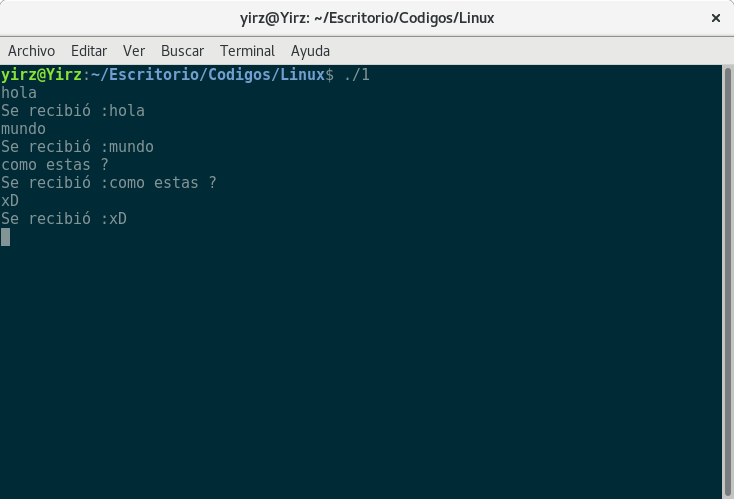
\includegraphics[scale=0.5]{Imagenes/Linux/1.png}
    \end{center}
    \item Aplicación que crea un procesos hijo a partir de un proceso padre, el proceso padre enviará al proceso hijo, a través de una tubería, dos matrices de 10x10 a multiplicar por parte del hijo, mientras tanto el proceso hijo creará un hijo de él, al cual enviará dos matrices de 10x10 a sumar en el proceso hijo creado, nuevamente el envió de estos valores será a través de una tubería. Una vez calculado el resultado de la suma, el proceso hijo del hijo devolverá la matriz resultante de la multiplicación que realizó a su abuelo(vía tuberia). A su vez, el proceso hijo devolverá la matriz resultante de la multiplicación que realizó a su padre. Finalmente, el lo guardará en un archivo para cada matriz inversa obtenida.
    
    \item Captura, compilación y ejecución de los siguientes programas.
    \lstinputlisting{Codigos/Linux/2.c}
    
    \lstinputlisting{Codigos/Linux/3.c}
     \begin{center}
		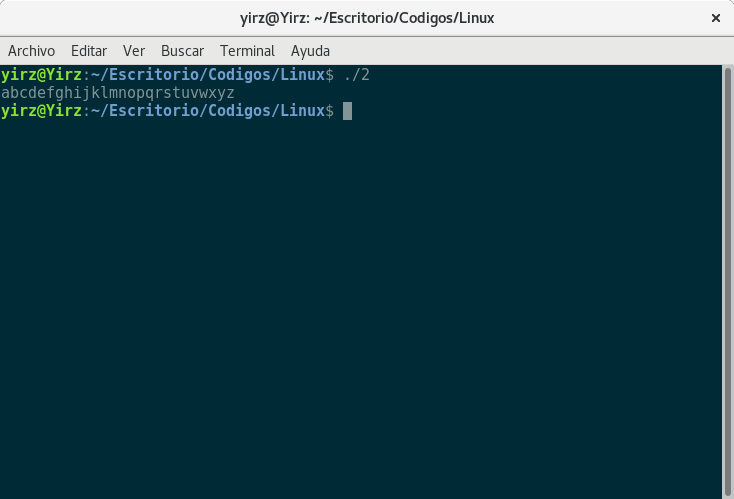
\includegraphics[scale=0.5]{Imagenes/Linux/2.png}
    \end{center}
     \begin{center}
		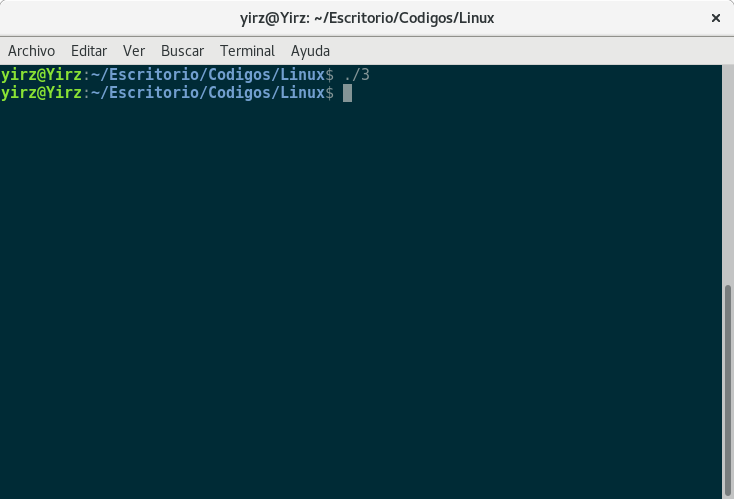
\includegraphics[scale=0.5]{Imagenes/Linux/3.png}
    \end{center}
    
     \item Aplicación anterior utilizando memoria compartida en lugar de tuberías.
    
    \end{enumerate}
    
\subsection{Windows}
\begin{enumerate}

    \item Captura, compilación y ejecución de los siguientes programas.
    \lstinputlisting{Codigos/Windows/4.c}
    
    \lstinputlisting{Codigos/Windows/5.c}\\
    \begin{center}
        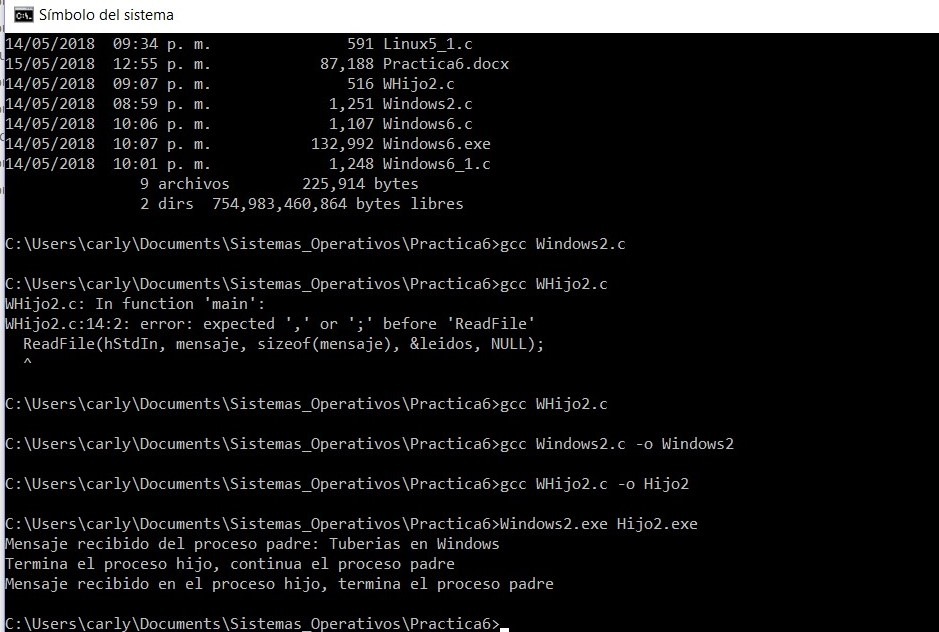
\includegraphics[scale=0.5]{Imagenes/Windows/4.jpg}
    \end{center}

    
    \item Aplicación que crea un procesos hijo a partir de un proceso padre, el proceso padre enviará al proceso hijo, a través de una tubería, dos matrices de 10x10 a multiplicar por parte del hijo, mientras tanto el proceso hijo creará un hijo de él, al cual enviará dos matrices de 10x10 a sumar en el proceso hijo creado, nuevamente el envió de estos valores será a través de una tubería. Una vez calculado el resultado de la suma, el proceso hijo del hijo devolverá la matriz resultante de la multiplicación que realizó a su abuelo(vía tuberia). A su vez, el proceso hijo devolverá la matriz resultante de la multiplicación que realizó a su padre. Finalmente, el lo guardará en un archivo para cada matriz inversa obtenida.
    
     \item Captura, compilación y ejecución de los siguientes programas.
    \lstinputlisting{Codigos/Windows/6.c}
    
    \lstinputlisting{Codigos/Windows/7.c}
    \begin{center}
        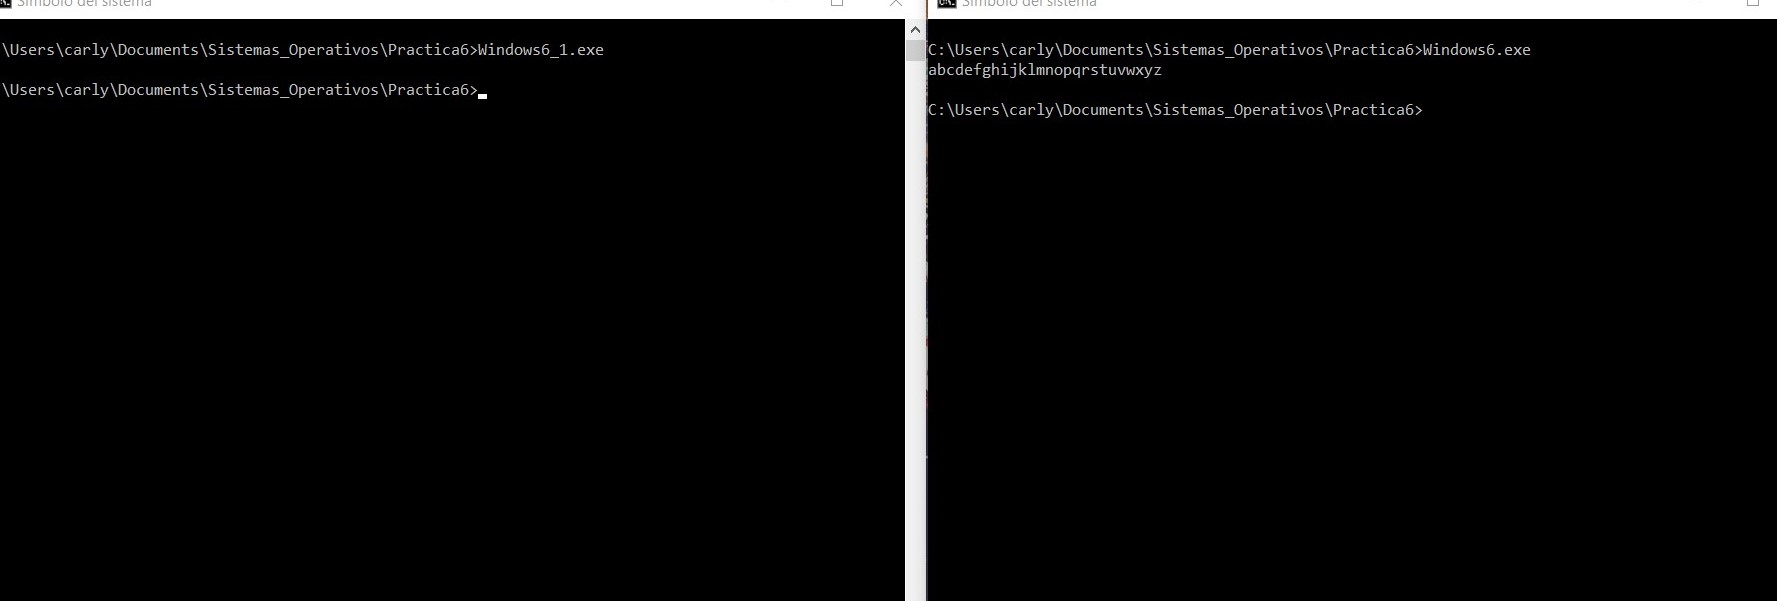
\includegraphics[scale=0.35]{Imagenes/Windows/6-Servidor.jpg}
    \end{center}
    \item Aplicación anterior utilizando memoria compartida en lugar de tuberías.
    
  
\end{enumerate}
\subsection{Programas Desarrollados}
    \subsubsection{Linux}
        \begin{itemize}
            \item \textbf{Tuberias}
            \begin{center}
                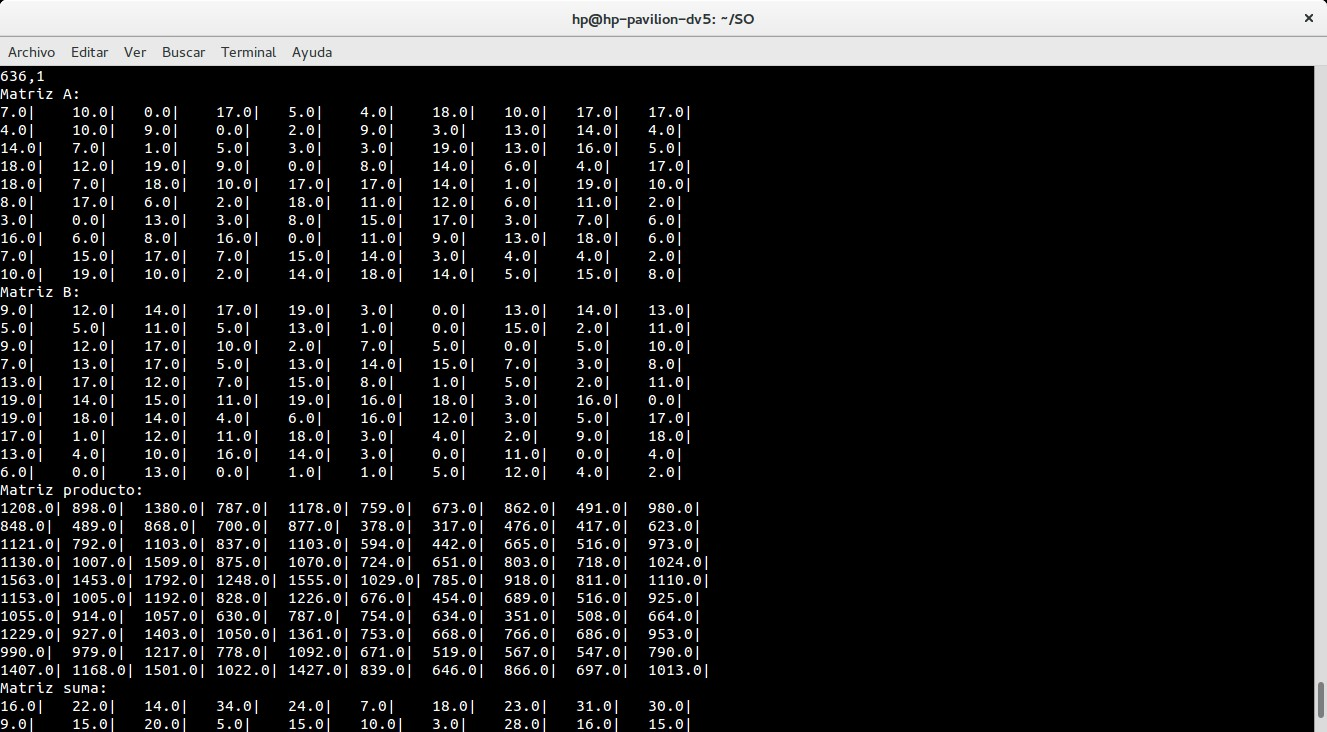
\includegraphics[scale=0.5]{Imagenes/Linux/10x10 (1).jpg}\\
                 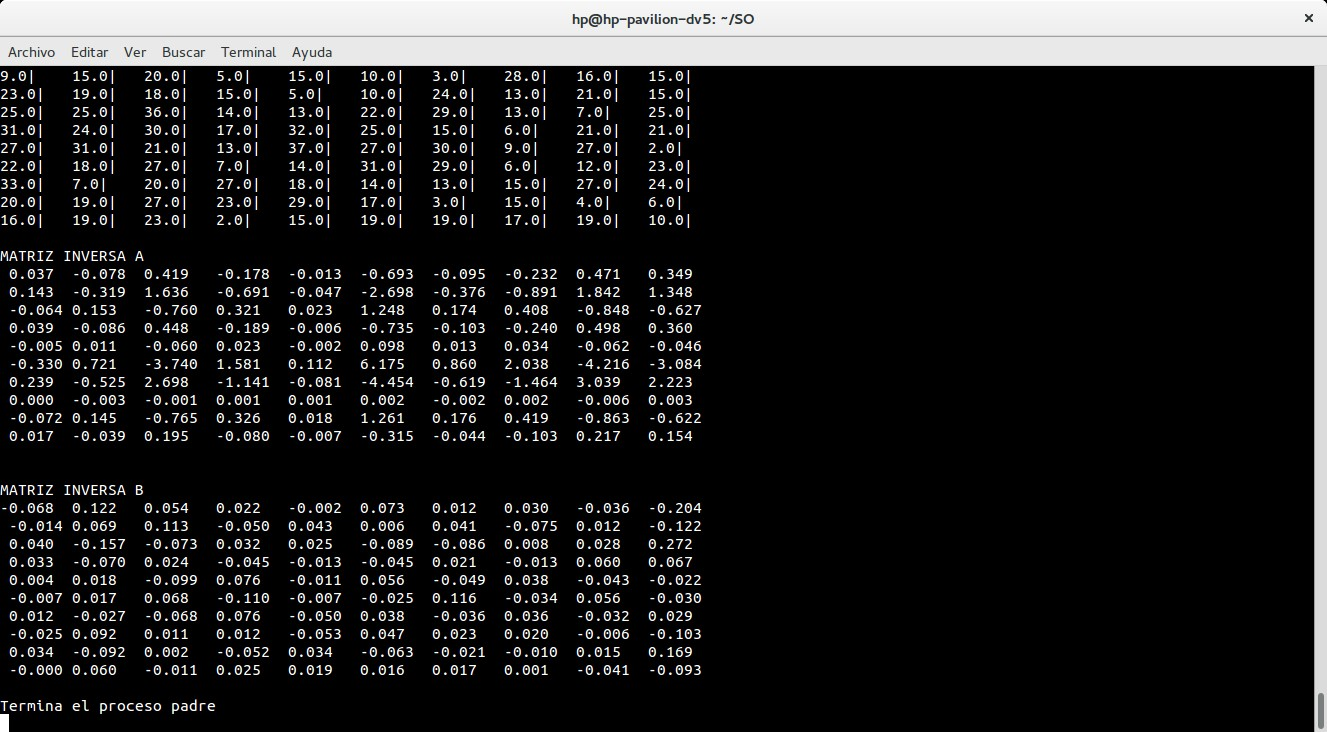
\includegraphics[scale=0.5]{Imagenes/Linux/10x10 (2).jpg}\\
                  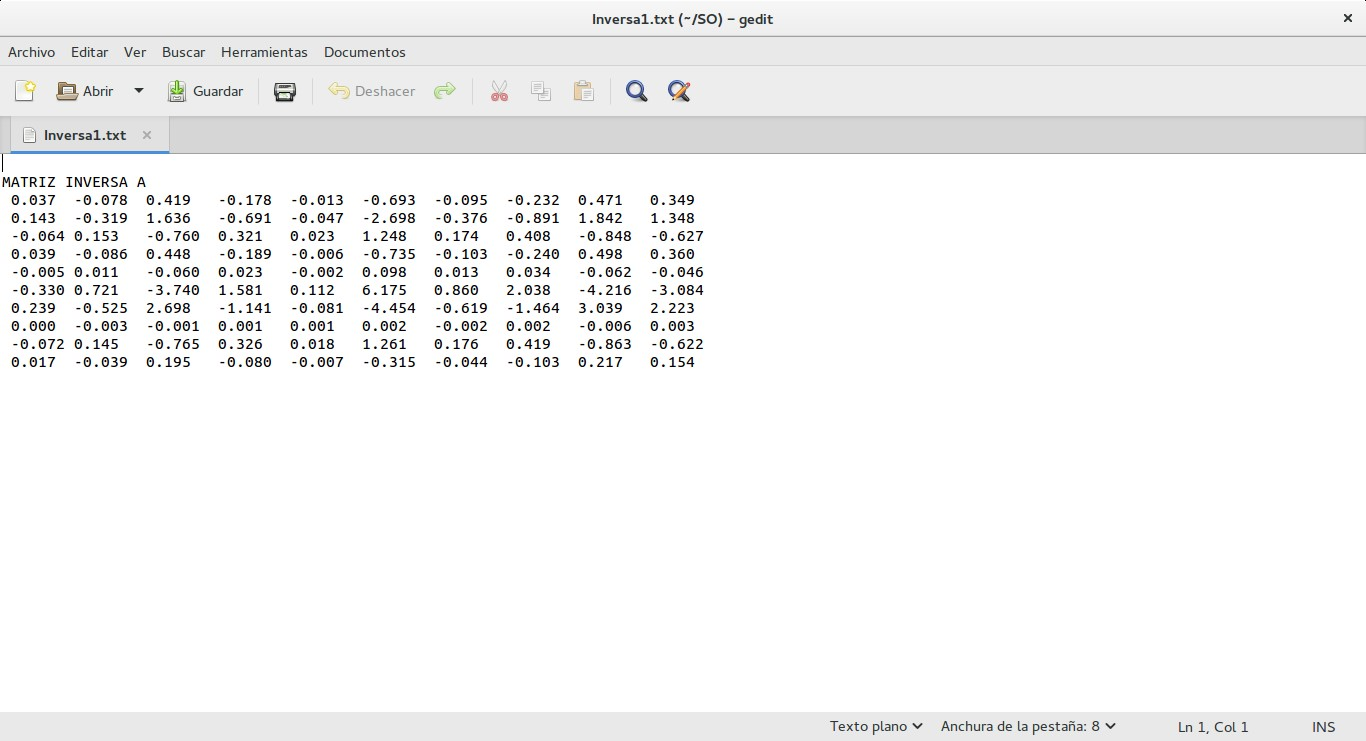
\includegraphics[scale=0.5]{Imagenes/Linux/10x10 (3).jpg}\\
                   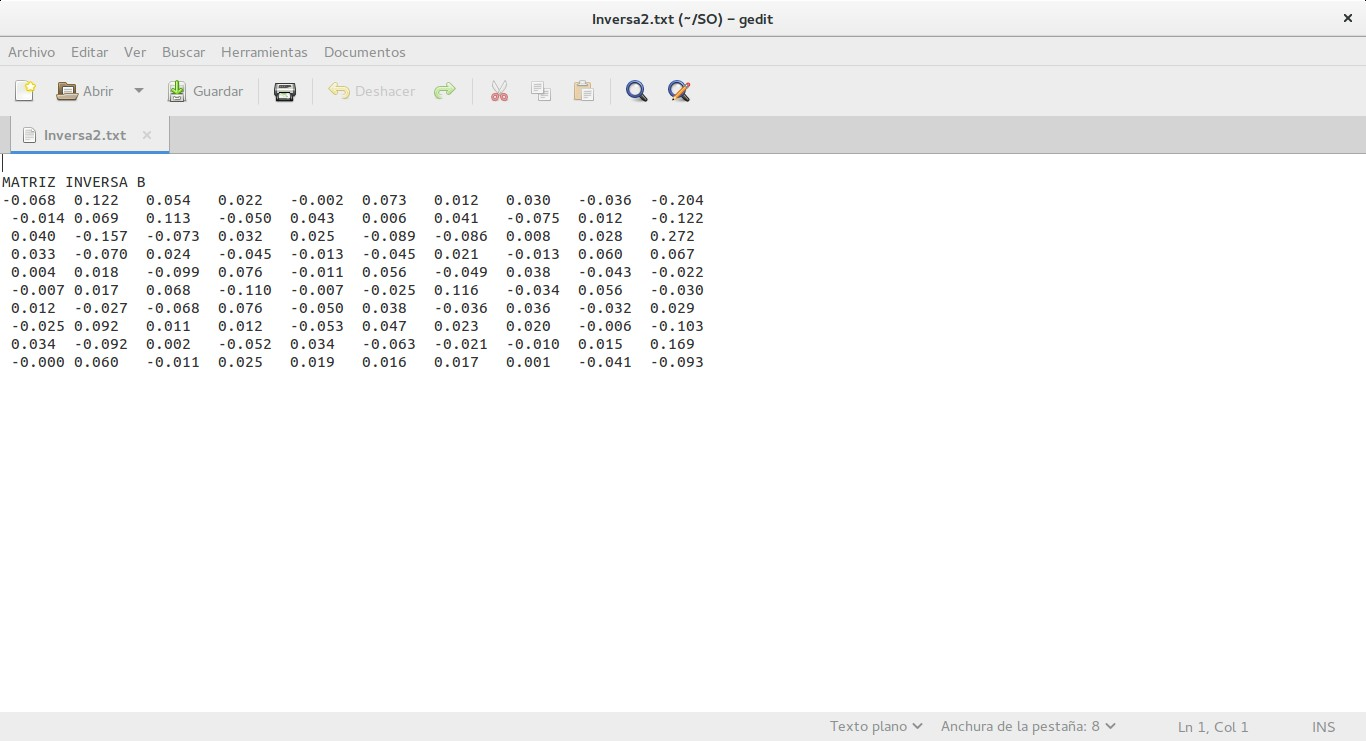
\includegraphics[scale=0.5]{Imagenes/Linux/10x10 (4).jpg}\\
            \end{center}
            \item \textbf{Memoria compartida}\\
            \begin{center}
                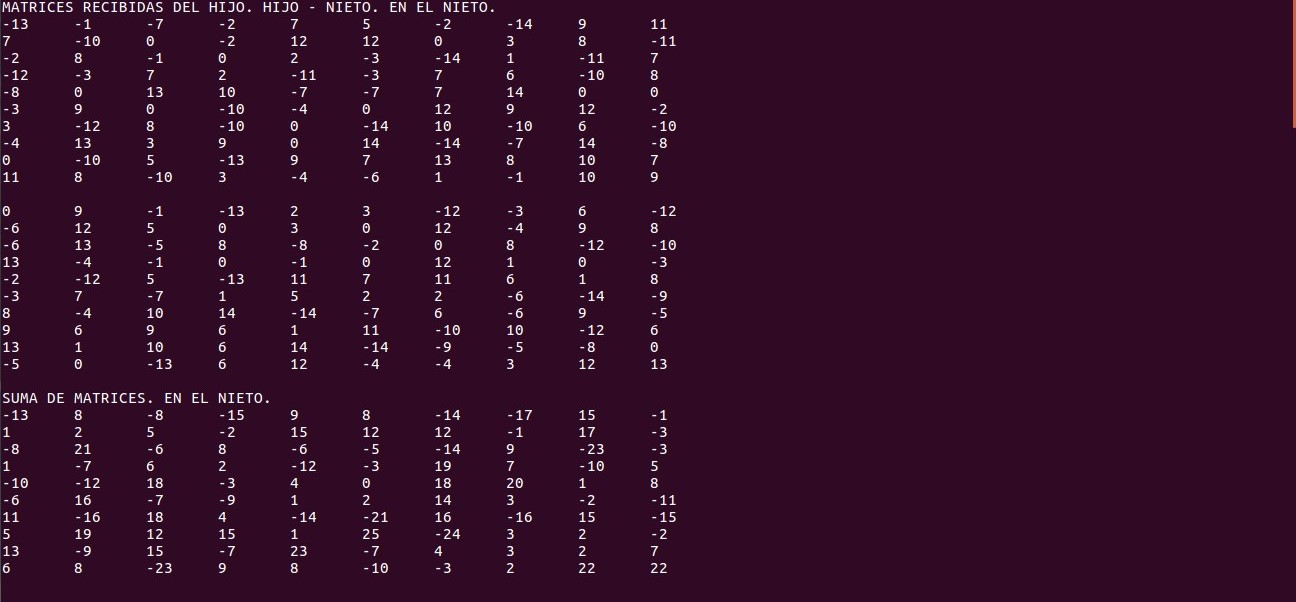
\includegraphics[scale=0.5]{Imagenes/Linux/padre,hijo, nieto (1).jpg}\\
                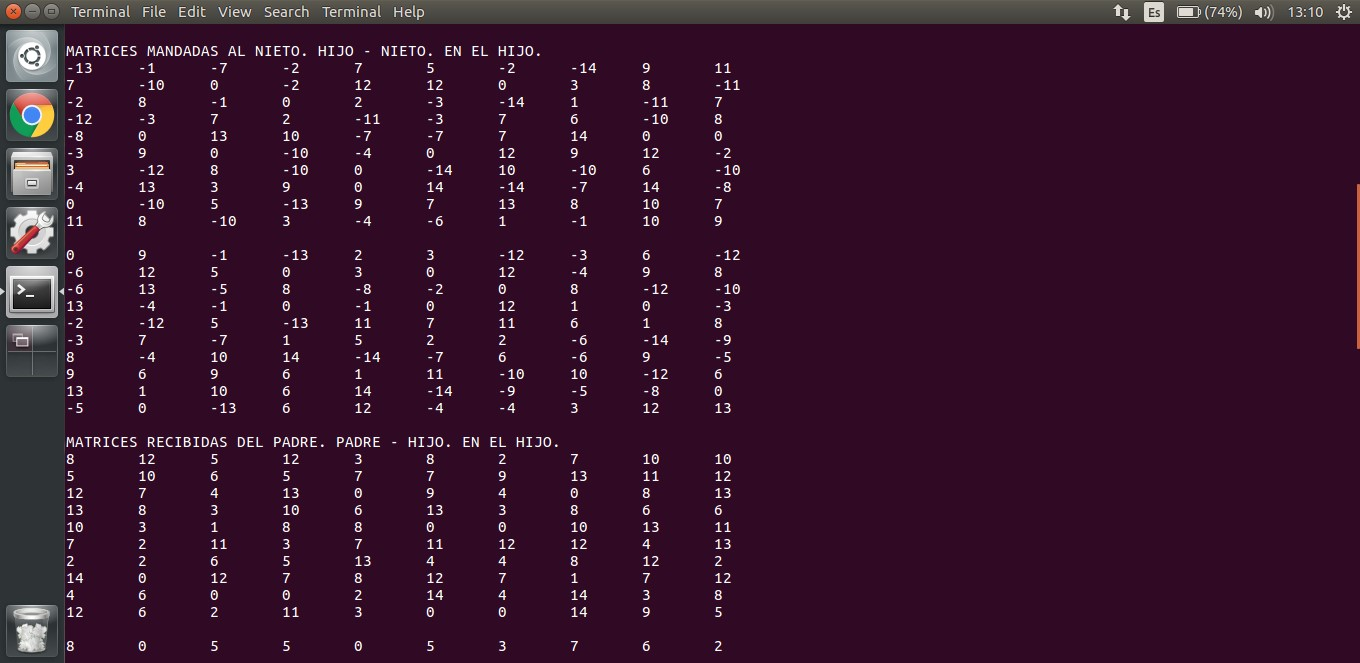
\includegraphics[scale=0.4]{Imagenes/Linux/padre,hijo, nieto (2).jpg}\\
                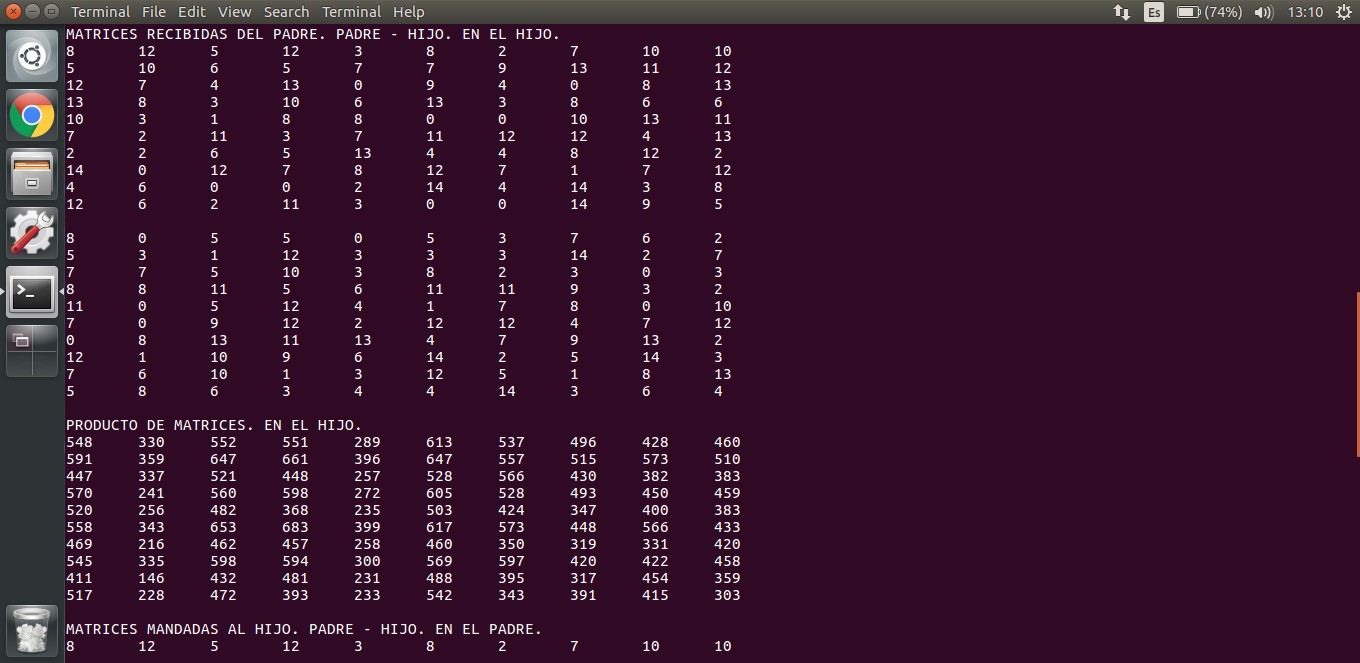
\includegraphics[scale=0.4]{Imagenes/Linux/padre,hijo, nieto (3).jpg}\\
                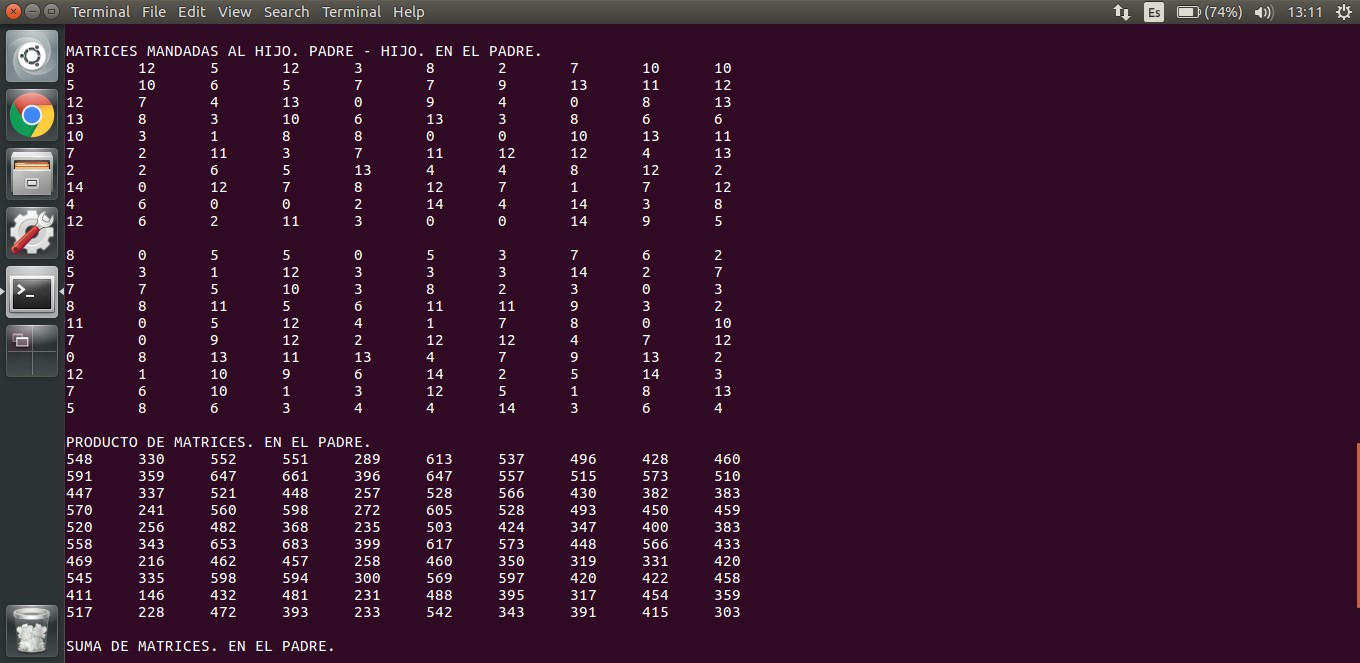
\includegraphics[scale=0.4]{Imagenes/Linux/padre,hijo, nieto (4).jpg}\\
                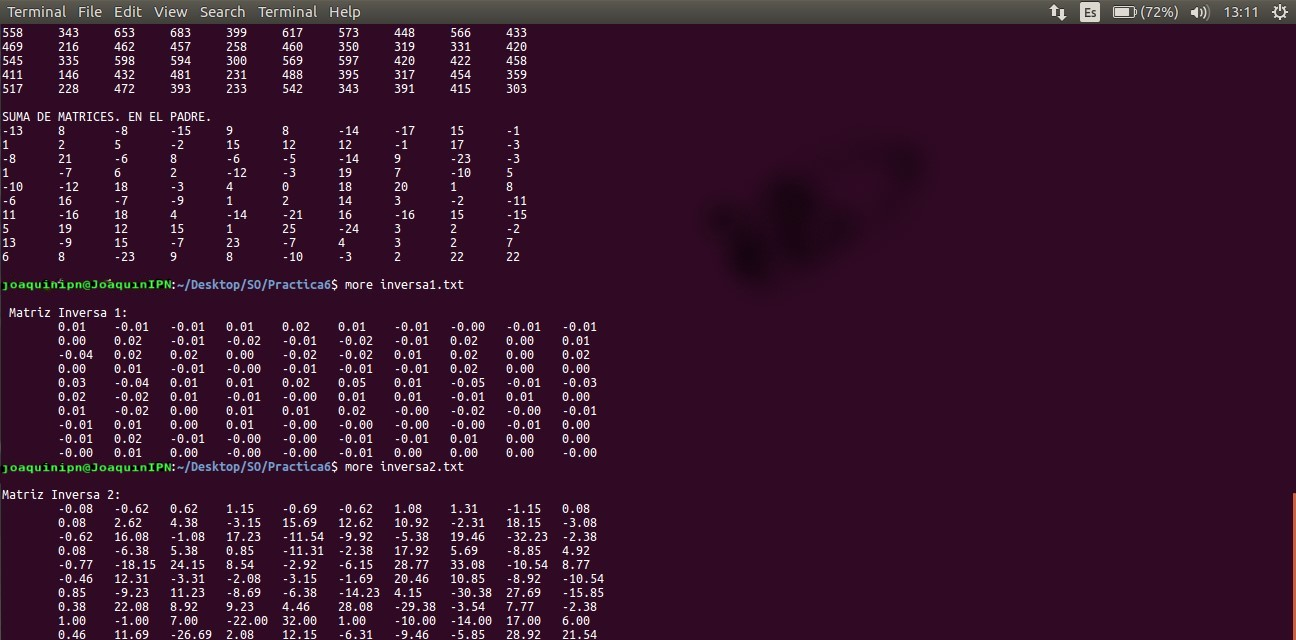
\includegraphics[scale=0.5]{Imagenes/Linux/padre,hijo, nieto (5).jpg}\\
            \end{center}
        \end{itemize}
    \subsubsection{Windows}
        \begin{itemize}
            \item \textbf{Tuberias}
            \begin{center}
                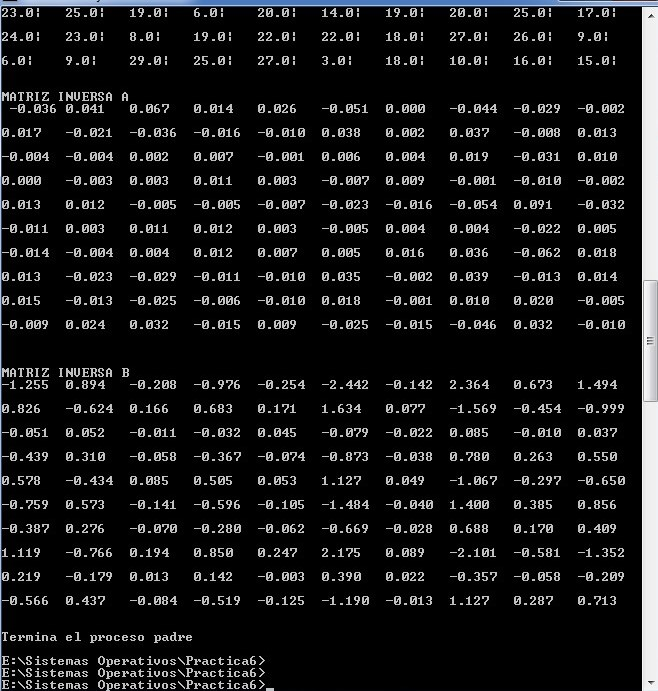
\includegraphics[scale=0.5]{Imagenes/Windows/10x10W (1).jpg}\\
                 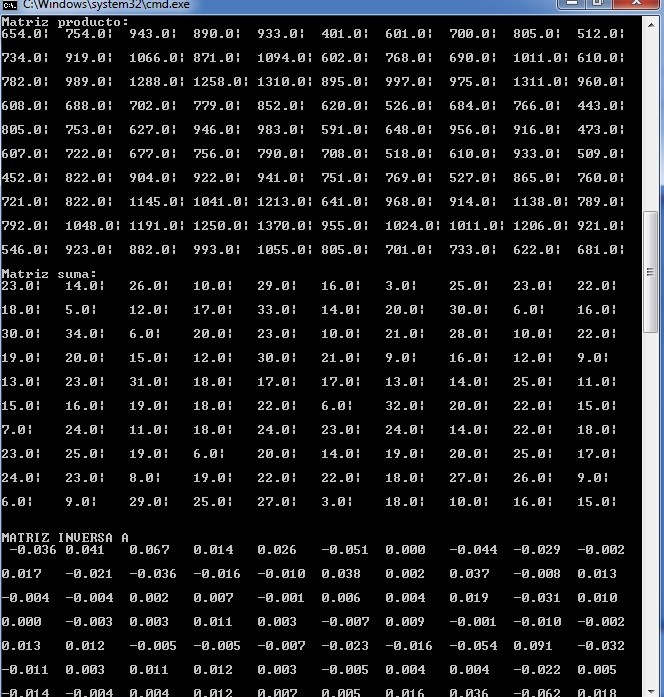
\includegraphics[scale=0.5]{Imagenes/Windows/10x10W (2).jpg}\\
                  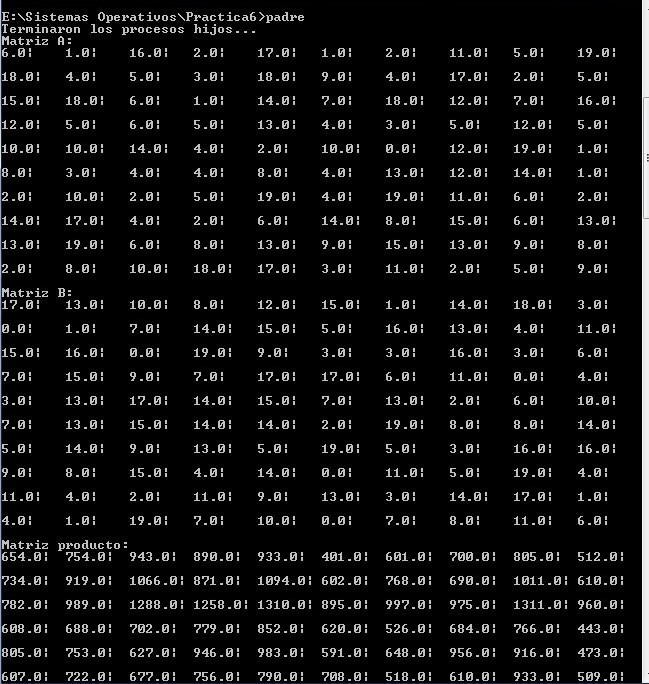
\includegraphics[scale=0.5]{Imagenes/Windows/10x10W (3).jpg}\\
                   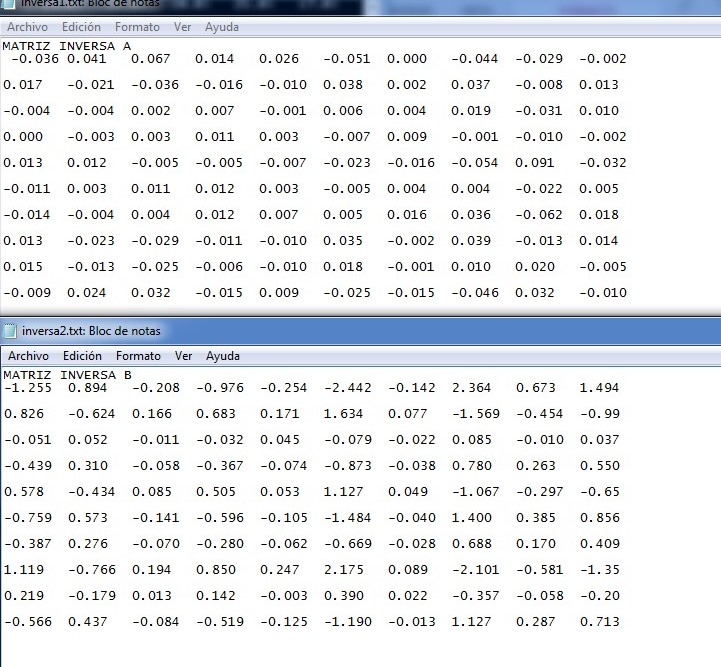
\includegraphics[scale=0.5]{Imagenes/Windows/10x10W (4).jpg}\\
                  
            \end{center}
            \item \textbf{Memoria compartida}\\
            \begin{center}
                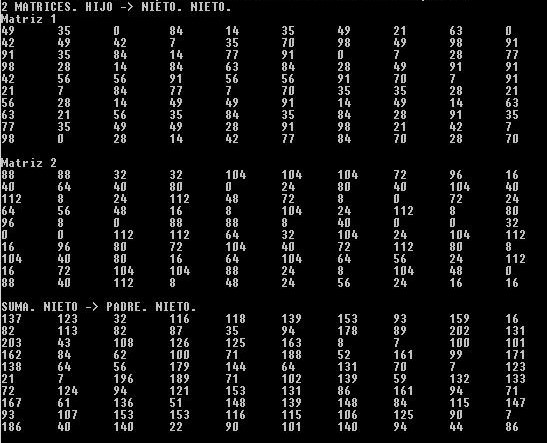
\includegraphics[scale=0.5]{Imagenes/Windows/prueba1,2.jpg}\\
               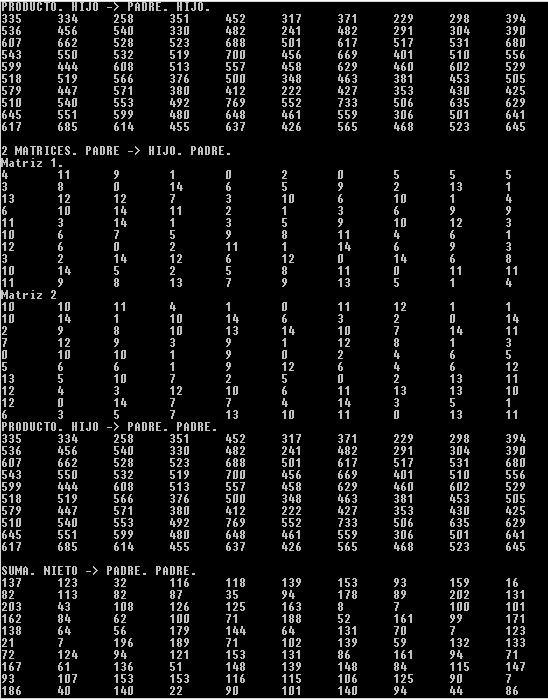
\includegraphics[scale=0.5]{Imagenes/Windows/prueba1,2 (1).jpg}\\
                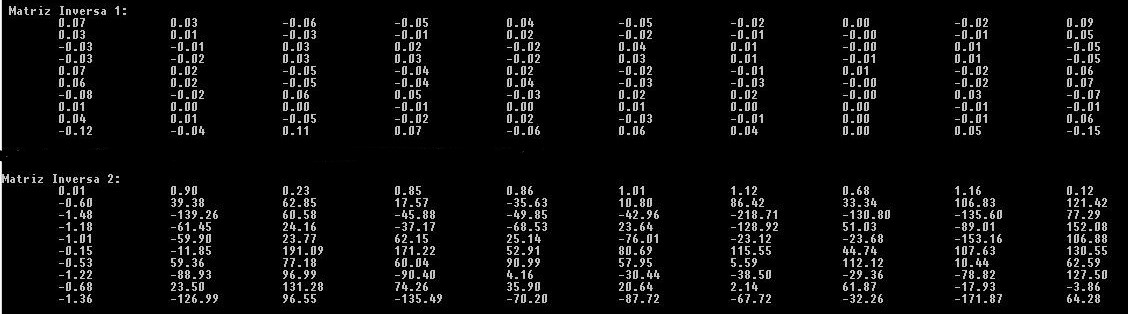
\includegraphics[scale=0.5]{Imagenes/Windows/prueba 1,2 (2).jpg}
                
            \end{center}
        \end{itemize}
\subsection{Código Fuente.}
   \subsubsection{Linux}
   Problema 3:
   
   \lstinputlisting{Codigos/Linux/10x10.c}
    
    Problema 5:
    
    Padre:
   \lstinputlisting{Codigos/Linux/padre.c}
   Hijo:
   \lstinputlisting{Codigos/Linux/hijo.c}
   Nieto:
   \lstinputlisting{Codigos/Linux/nieto.c}
        
   \subsubsection{Windows}
   Problema 3:
   
   \lstinputlisting{Codigos/Windows/10x10W.c}
   
   Problema 5:
   
   \lstinputlisting{Codigos/Windows/prueba1.c}
   
   \lstinputlisting{Codigos/Windows/prueba2.c}
 
   
  
   


\section{Observaciones.}
Se realiza todo lo que se pide en la práctica utilizando tuberías, solo que de forma unidireccional, notamos que en linux es muy sencillo llevar el control de las tuberías en ambos sentidos pero en windows es algo mucho más complejo, ya que al intentar hacer el intercambio de información de forma bidireccional el programa se tilda, eso se debe a que el programa espera a recibir la información pero no lo hace, probablemente fue algún error con el manejo de la información, recordemos que una tubería solo tiene una sola dirección y si quisiéramos realizar la comunicación mutua con alguno de sus descendientes en linux es muy sencillo, solo que windows al manejar bastantes controles de seguridad no permite que sea tan cómodo.\\

En caso de windows se realizó 3 programas el primero es el servidor el cual genera los datos de la matriz y los guarda en dos memorias dinámicas para cada  matriz, con la ayuda de apuntadores y con el corrimiento de las direcciones de memoria pudimos realizar la manipulación de información. en el segundo programa se accedió a los primeros dos bloques para guardar  la suma en un tercer bloque, en el tercer programa se usó los mismos dos bloques los cuales se usaron para multiplicarlos y guardarlos en una cuarta matriz. Finalmente el programa servidor accedía al tercer bloque y al cuarto para calcular la inversa y mostrar el resultado en consola y en un archivo de texto.
El control de memoria se realizó con la ayuda de una función llamada “espera”, lo que realizaba es que el proceso se esperará hasta que el primer bloque de alguna memoria  fuera -1 , esto era escrito por algún proceso que lo esté ocupando y para evitar la pérdida del bloque de memoria.



\section{Análisis Crítico.}

La realización de esta práctica fue un poco más compleja que la parte de realización de procesos, sin embargo, en ésta debemos de utilizar la comunicación entre procesos. En la parte de memoria compartida se investigaron algunas funciones y la manera en que se trasladaban las funciones. En general, nos fue más sencillo el crear las aplicaciones en lo que es el sistema operativo de Linux.

\section{Conclusión.}

Con la práctica pudimos observar y llevar a su funcionamiento la teoría vista en clase. Como ya vimos, la memoria compartida, en pocas palabras, significa utilizar una parte de la memoria física y por así decir, volverla memoria virtual, esto a través de la paginación. Al momento de capturar y analizar los códigos ejemplo, en el caso de las tuberías, observe que en una tubería solamente los datos pueden ir en una sola dirección. Por lo tanto, en una tubería normal, se usa un método que es para la escritura y otro método para la lectura pero en dado caso de que quisiéramos mandar informacion en sentido contrario (imaginando la tuberia, ir de izquierda a derecha y viceversa) entonces tendríamos que hacer uso de 2 tuberías, las cuales una ira de izquierda a derecha y la otra de derecha a izquierda, cada una de las tuberías con sus dos métodos para escribir y leer.

\end{document}